\chapter{Results and Discussion}

\section{Dimensional and Non-Dimensional Simulations}

The problem has a initial condition for interface of the droplet at a height $H_o$ from the bottom of the domain. It can be seen that both dimensional and non-dimensional simulation 
interface overlaps each other (See Fig 5.1 - 5.4) 



\begin{figure}
\def\tabularxcolumn#1{m{#1}}
\begin{tabularx}{\linewidth}{@{}cXX@{}}
%
\begin{tabular}{cc}
\centering
\subfloat[t = 0]{\includegraphics[scale=0.4]{Hung_D_ND-0.eps}} 
   & \subfloat[t = 0.01]{\includegraphics[scale=0.4]{Hung_D_ND-0.01.eps}}\\
\subfloat[t = 0.02]{\includegraphics[scale=0.4]{Hung_D_ND-0.02.eps}} 
   & \subfloat[t = 0.03]{\includegraphics[scale=0.4]{Hung_D_ND-0.03.eps}}\\
\subfloat[t = 0.04]{\includegraphics[scale=0.4]{Hung_D_ND-0.04.eps}} 
   & \subfloat[t = 0.05]{\includegraphics[scale=0.4]{Hung_D_ND-0.05.eps}}\\
    \subfloat[t = 0.06]{\includegraphics[scale=0.4]{Hung_D_ND-0.06.eps}}
   & \subfloat[t = 0.07]{\includegraphics[scale=0.4]{Hung_D_ND-0.07.eps}}\\
\end{tabular}
\end{tabularx}
\caption{Comparison of Dimensional(Blue) and Non-Dimensional(Red) simulations in Gerris (t = Dimensional time in seconds)}
\end{figure}


\begin{figure}
\def\tabularxcolumn#1{m{#1}}
\begin{tabularx}{\linewidth}{@{}cXX@{}}
%
\begin{tabular}{cc}
  \subfloat[t = 0.08]{\includegraphics[scale=0.4]{Hung_D_ND-0.08.eps}}
   & \subfloat[t = 0.09]{\includegraphics[scale=0.4]{Hung_D_ND-0.09.eps}}\\
    \subfloat[t = 0.10]{\includegraphics[scale=0.4]{Hung_D_ND-0.1.eps}}
   & \subfloat[t = 0.11]{\includegraphics[scale=0.4]{Hung_D_ND-0.11.eps}}\\
    \subfloat[t = 0.12]{\includegraphics[scale=0.4]{Hung_D_ND-0.12.eps}}
   & \subfloat[t = 0.13]{\includegraphics[scale=0.4]{Hung_D_ND-0.13.eps}}\\
    \subfloat[t = 0.14]{\includegraphics[scale=0.4]{Hung_D_ND-0.14.eps}}
   & \subfloat[t = 0.15]{\includegraphics[scale=0.4]{Hung_D_ND-0.15.eps}}
\end{tabular}
\end{tabularx}
\caption{Comparison of Dimensional(Blue) and Non-Dimensional(Red) simulations in Gerris (t = Dimensional time in seconds)}
\end{figure}


\begin{figure}
\def\tabularxcolumn#1{m{#1}}
\begin{tabularx}{\linewidth}{@{}cXX@{}}
%
\begin{tabular}{cc}
  \subfloat[t = 0.16]{\includegraphics[scale=0.4]{Hung_D_ND-0.16.eps}}
   & \subfloat[t = 0.17]{\includegraphics[scale=0.4]{Hung_D_ND-0.17.eps}}\\
    \subfloat[t = 0.18]{\includegraphics[scale=0.4]{Hung_D_ND-0.18.eps}}
   & \subfloat[t = 0.19]{\includegraphics[scale=0.4]{Hung_D_ND-0.19.eps}}\\
    \subfloat[t = 0.20]{\includegraphics[scale=0.4]{Hung_D_ND-0.2.eps}}
   & \subfloat[t = 0.21]{\includegraphics[scale=0.4]{Hung_D_ND-0.21.eps}}\\
    \subfloat[t = 0.22]{\includegraphics[scale=0.4]{Hung_D_ND-0.22.eps}}
   & \subfloat[t = 0.23]{\includegraphics[scale=0.4]{Hung_D_ND-0.23.eps}}
\end{tabular}
\end{tabularx}
\caption{Comparison of Dimensional(Blue) and Non-Dimensional(Red) simulations in Gerris (t = Dimensional time in seconds)}
\end{figure}

\begin{figure}
\def\tabularxcolumn#1{m{#1}}
\begin{tabularx}{\linewidth}{@{}cXX@{}}
%
\begin{tabular}{cc}
  \subfloat[t = 0.24]{\includegraphics[scale=0.4]{Hung_D_ND-0.24.eps}}
   & \subfloat[t = 0.25]{\includegraphics[scale=0.4]{Hung_D_ND-0.25.eps}}\\
    \subfloat[t = 0.26]{\includegraphics[scale=0.4]{Hung_D_ND-0.26.eps}}
   & \subfloat[t = 0.27]{\includegraphics[scale=0.4]{Hung_D_ND-0.27.eps}}\\
    \subfloat[t = 0.28]{\includegraphics[scale=0.4]{Hung_D_ND-0.28.eps}}
   & \subfloat[t = 0.29]{\includegraphics[scale=0.4]{Hung_D_ND-0.29.eps}}\\
    \subfloat[t = 0.30]{\includegraphics[scale=0.4]{Hung_D_ND-0.3.eps}}
   & \subfloat[t = 0.31]{\includegraphics[scale=0.4]{Hung_D_ND-0.31.eps}}
\end{tabular}
\end{tabularx}
\caption{Comparison of Dimensional(Blue) and Non-Dimensional(Red) simulations in Gerris (t = Dimensional time in seconds)}
\end{figure}

\section{Comparison of Gerris simulation with experiment}
The interface points from the experimental data(\cite{Hung2011}) has been extracted and compared with Gerris simulation data. 
The simulation results were in agreement with experiment before the impact. Just after the impact (See Fig 5.5 (a),(b)) the contact line and the contact angle is coinciding with 
the experimental but as the contact line started to move in the (c) \& (d), the simulation interface did not moved because of the no slip boundary condition and also has the contact 
contact angle. From (c) to (j) the results are very different from what is observed in the experiment.

\begin{figure}[tpb]
\centering
 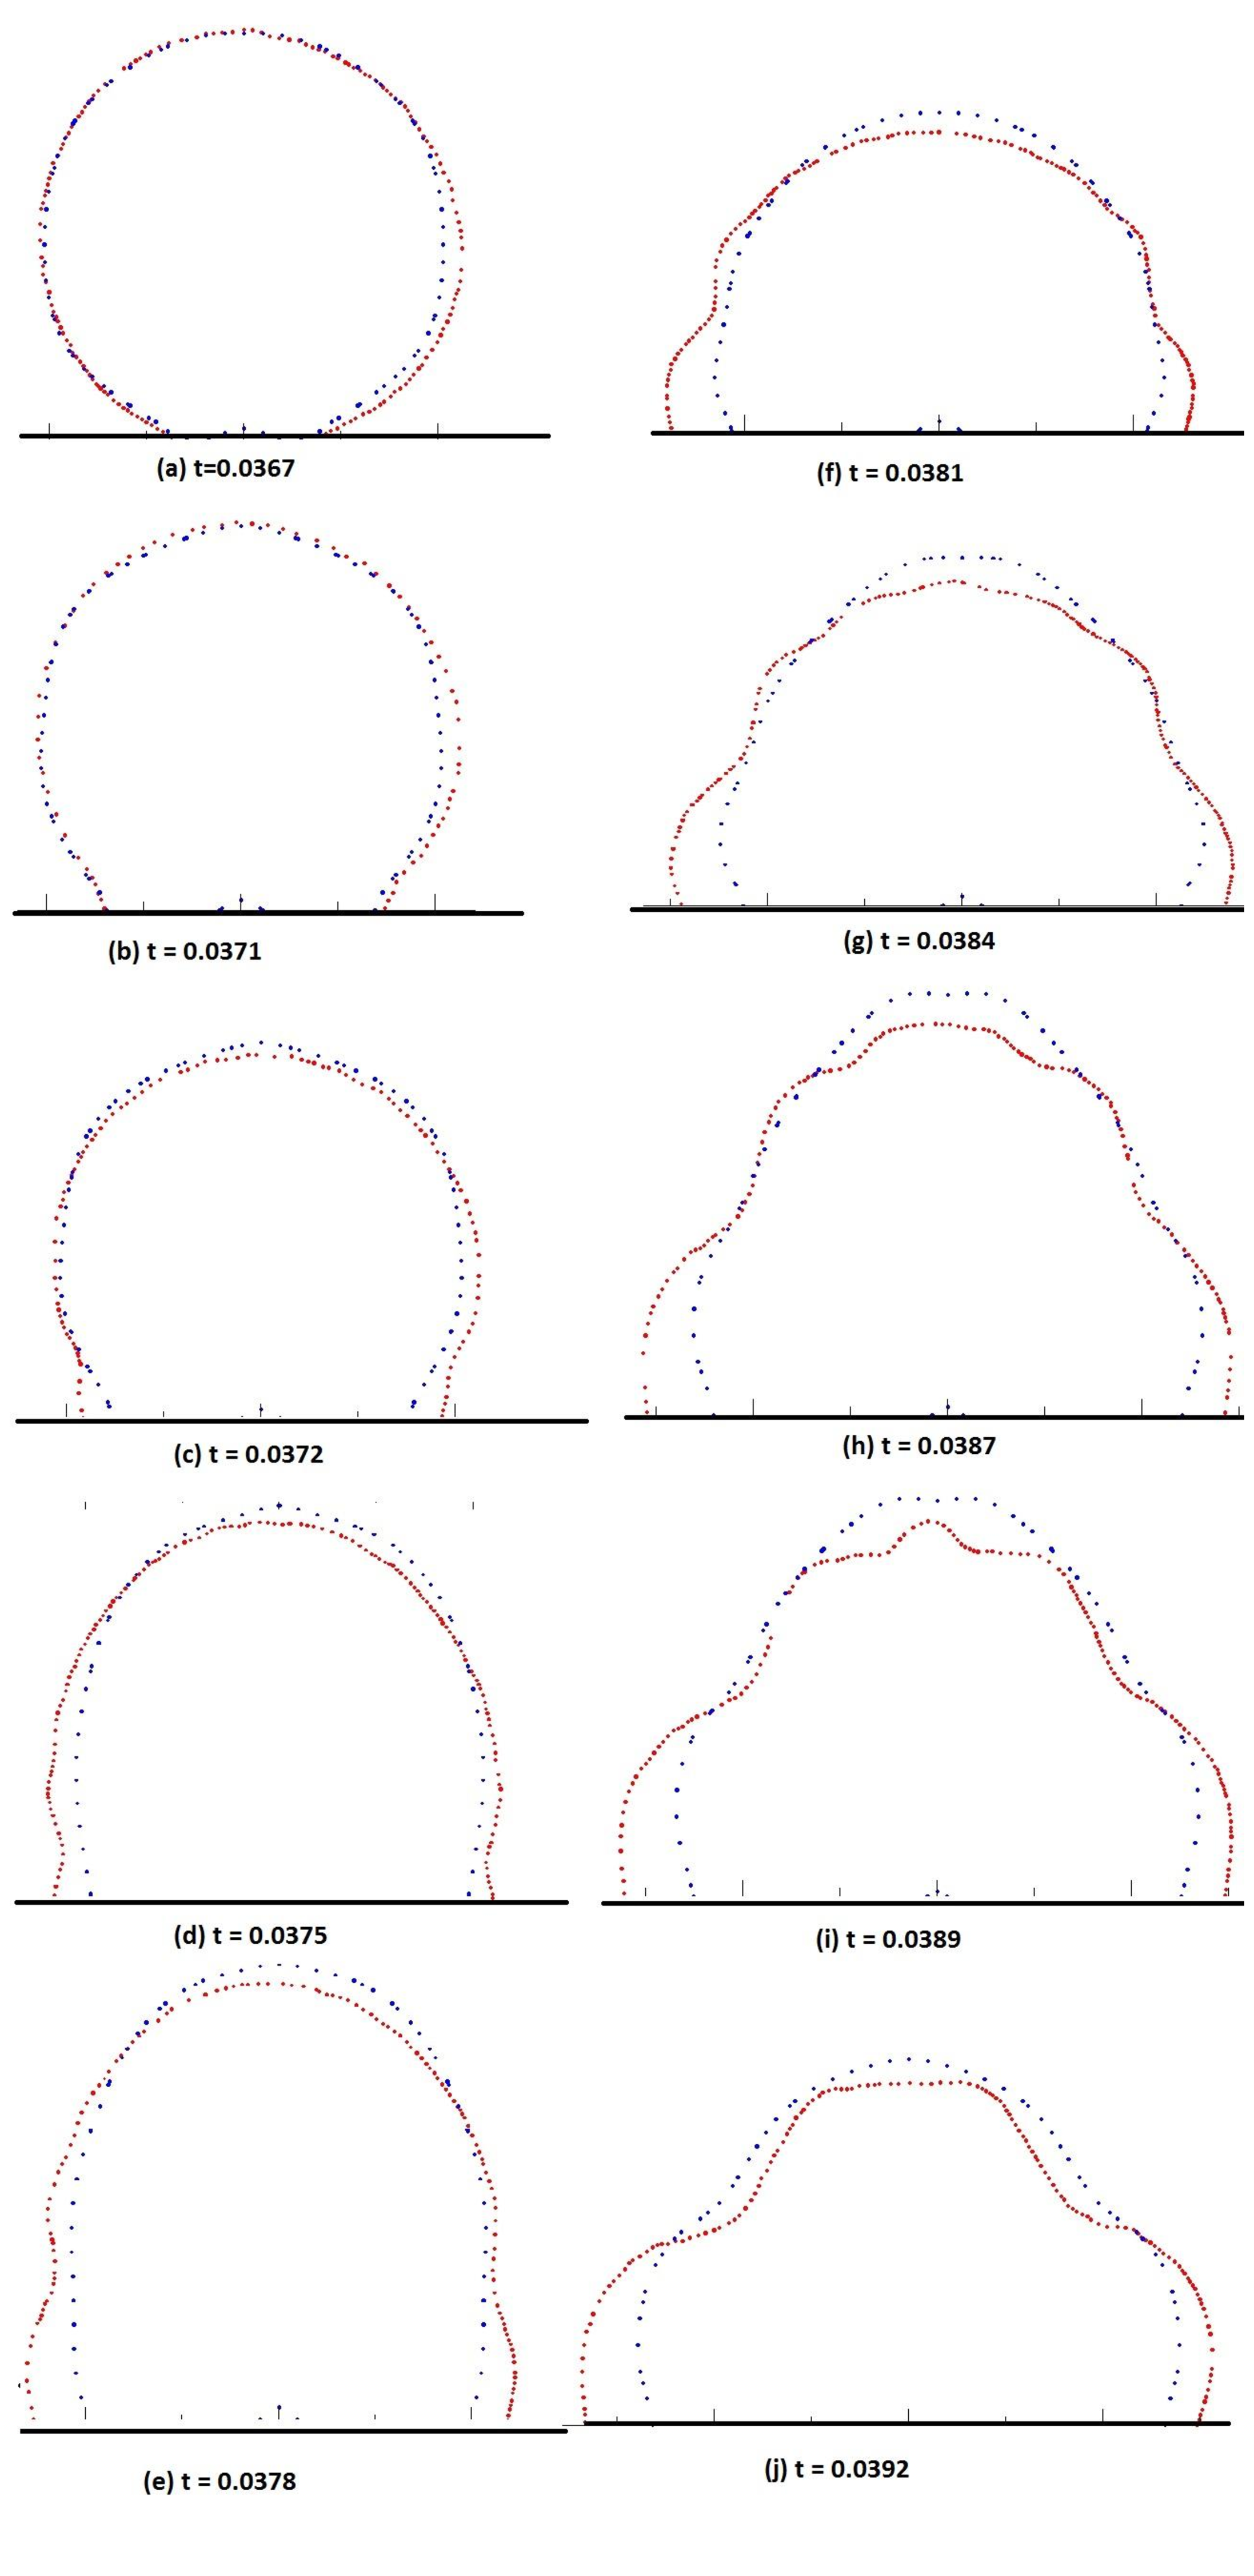
\includegraphics[scale=0.3]{hung.eps}
 \caption{Comparison Gerris simulation data(BLUE) with \cite{Hung2011} experimental data(RED)}
\end{figure}

\section{Conclusion}
Due to this limitation of Gerris code, Our future work involves development of a multiphase Navier-Stokes solver and to implement the moving contact line and dynamic contact line model in it, 
Till then we will use Gerris code to observed some simpler outcomes of droplet impact. Our code will mimic the actual droplet impact after implementation of the contact models. We also
look to explain some aspects of this phenomena through a simpler mathematical model.
